\pdfinfo{
/ModDate (\pdfcreationdate)                                   
/Producer (pdfLaTeX)                                    
}


\documentclass[fleqn,oneside,openany,a4paper,11pt]{book}

\usepackage{color}
\usepackage[utf8]{inputenc}
\usepackage[breaklinks]{hyperref} %
\usepackage{pracadok}
\usepackage{longtable}
\usepackage{array}
\usepackage{geometry}
\usepackage{fancyhdr}
\usepackage{float}
\usepackage{verbatim}
\pdfcompresslevel=9

\def\uwaga#1{}

\begin{document}
\let\s\lstinline
\lstset{inputencoding=utf8, extendedchars=true,literate={ą}{{\k{a}}}1 {ć}{{\'c}}1 {ę}{{\k{e}}}1 {ł}{{\l{}}}1 {ń}{{\'n}}1 {ó}{{\'o}}1 {ś}{{\'s}}1 {ż}{{\.z}}1 {ź}{{\'z}}1 {Ą}{{\k{A}}}1 {Ć}{{\'C}}1 {Ę}{{\k{E}}}1 {Ł}{{\L{}}}1 {Ń}{{\'N}}1 {Ó}{{\'O}}1 {Ś}{{\'S}}1 {Ż}{{\.Z}}1 {Ź}{{\'Z}}1}

% Tytuł
\def\autor{Informatyka Stosowana III rok}
\def\tytul{\textbf{\LARGE Projektowanie bazy danych}}
\def\promotor{~}
\def\miejscerokwydania{Nowy Sącz \today}
\def\nazwauczelni{PAŃSTWOWA WYŻSZA SZKOŁA ZAWODOWA}
\def\imienia{INSTYTUT  TECHNICZNY}
\def\wydzial{Kierunek Informatyka Stosowana}

\thispagestyle{empty}
{
\hbox{}\vskip 0.3\textheight
\hspace{1cm}
\centering
\vbox{
\noindent\textbf{\Huge Projekt bazy danych \\ \vspace{0.3cm}sklepu internetowego}\vspace{0.5cm}\\
\noindent\textbf{\vspace{0.3cm}Bazy danych}\\
\noindent\textbf{Prowadzący: Antoni Ligęza}}\\}
%\noindent e-mail: \verb|aligeza@pwsz-ns.edu.pl|\\
%\noindent \verb|http://www.pwsz-ns.edu.pl/aligeza|}\\}
\definecolor{tlo}{rgb}{.7,.7,.7} 
\lstset{language=bash,commentstyle=\scriptsize,backgroundcolor=\color{tlo},%
basicstyle=\scriptsize}

%spis tresci
{\footnotesize\tableofcontents}

\setcounter{chapter}{0}
\chapter{Projektowanie Bazy Danych}
Projekt: Przygotowanie Systemu Zarządzania Bazą Danych (dalej SZBD) zawierającego interfejs i bazę danych dla sklepu internetowego zajmującego się sprzedażą akcesorii kuchenych\\
Obecnie zamawiający SZBD sprzedaje towar na popularnym serwisie aukcyjnym.\\ 
\section{Sformułowanie celu i zadań}
\begin{enumerate}
\item Minimalizacja czasu
\begin{itemize}
\item pomiędzy złożeniem zamówienia przez klienta a przekazaniem towaru do wysyłki w przypadku wysyłki za pobraniem
\item pomiędzy zaksięgowaniem wpłaty klienta a przekazaniem towaru do wysyłki w przypadku płatności z góry 
\end{itemize} 
\item Minimalizacja ilości osób zaangażowanych w zarządzanie sprzedażą
\item Ujednolicenie istniejącej bazy produktów i ich kategorii
\item Uniezależnienie się od wykorzystywanego portalu aukcyjnego
\item Automatyzacja wystawiania faktur/rachunków
\item Zapewnienie łatwej kontroli nad aktualnymi stanami magazynowymi produktów
\item Zapewnienie kontroli dostępu do danych
\item Ograniczenie modyfikacji danych dla poszczególnych pracowników 
\end{enumerate}

\subsection{Analiza istniejacej bazy — analiza stanu wyjsciowego}
Zamawiający SZBD sprzedaje towar na popularnym serwisie aukcyjnym. 
Ze względu na powiększenie oferowanego asortymentu istniejący model funkcjonowania przedsiębiorstwa przestaje być wystarczająco wydajny 
ze względu na źle przemyślany schemat przechowywania danych
\begin{enumerate}
\item Opisy produktów jako pliki tekstowe przechowywane w strukturze katalogowej odpowiadającej kategoriom
\item Stany magazynowe w arkuszu kalkulacyjnym (bez multidostępu do zapisu)
\item Ceny w arkuszu kalkulacyjnym
\item Rozliczenia roczne w arkuszu kalkulacyjnym 
\item Dokumenty tj. faktury, raporty z przekazania do wysyłki) w formie papierowej
\item Baza kupujących przechowywana jest przez system aukcyjny	
\end{enumerate}
\textbf{W jaki sposób baza jest wykorzystywana?}\\
Aby dodać produkt do sprzedaży, wyszukiwany jest odpowiedni plik tekstowy z jego opisem oraz sprawdzane cena i stan magazynowy w arkuszu kalkulacyjnym.
Kategoria ustalana jest ręcznie w arkuszu kalulacyjnym zawierającym stany magazynowe
Produkty są wystawianie ręcznie na popularnym serwisie aukcyjnym.
Informacje o kupnie: jaki towar, w jakiej ilości, w jakiej cenie oraz o wpłacie dostarczane są przez serwis aukcyjny w formie tekstowej (elektronicznie)
Do osoby odpowiedzalnej za gromadzenie towaru w paczkę do wysyłki i przekazanie paczki kurierowi przekazywana jest w formie wydruku
Informacje potrzebne do generowania raportów przepisywane są do arkusza kalkulacyjnego ręcznie.\\
Problemy: 
\begin{enumerate}
	\item Dane wyszukiwane są ręcznie.
	\item Duże ryzyko błędu ludzkiego podczas ręcznego przenoszenia danych. 
\end{enumerate}


\subsection{Lista tabel w projektowanej bazie}

\begin{enumerate}
\item \textbf{Kategoria:}

\begin{tabular}{|l|l|l|l|l|l|} \hline
	\textbf{Nazwa} & \textbf{Typ} & \textbf{Atrybuty} & \textbf{Null} & \textbf{Ustawienia} & \textbf{Dodatkowo} \\
	&&&&\textbf{domyslne}&\\
	\hline
	\# kategoria\_id&int(10)&unsigned&nie&brak&AUTO\_INCREMENT \\
	nazwa&varchar(30)& - &nie& nieznana& - \\
	FK id\_nadrzędnej&int(10)&unsigned&tak&null& - \\
	\hline
\end{tabular}

\begin{itemize}
	\item \# kategoria\_id - pole jednoznacznie identyfikujące kategorię
	\item nazwa - nazwa kategorii może się powtarzać ( np. podkategoria "pozostałe" w różnych kategoriach)
	\item FK id\_nadrzednej - id kategorii nadrzędnej, kategoriami poziomu najwyższego są te, gdzie id\_ nadrzędnej ma watrość NULL
\end{itemize}
\item \textbf{Klient:}

\begin{tabular}{|l|l|l|l|l|l|} \hline
	\textbf{Nazwa} & \textbf{Typ} & \textbf{Atrybuty} & \textbf{Null} & \textbf{Ustawienia} & \textbf{Dodatkowo} \\
	&&&&\textbf{domyslne}&\\
	\hline
	klient\_id&int(10)&unsigned&nie&brak&A\_INC \\
	typ&unum('p' 'f')& - &nie& p& - \\
	nazwisko&varchar(50)&-&tak&null& - \\
	imie&varchar(50)&-&tak&null&-\\
	NIP&bigint(20)&-&tak&null&-\\
	nazwa\_firmy&varchar(100)&-&tak&null&-\\
	dom\_adr\_wys&varchar(200)&-&tak&null&-\\
	login&varchar(50)&-&nie&brak&-\\
	haslo&varchar(32)&-&nie&brak&-\\
	\hline
\end{tabular}
\begin{itemize}
	\item \# klient\_id, - pole jednoznacznie identyfikujące klienta
	\item typ - 'p'- klient indywidualny 'f' -firma
	\item nazwisko -
	\item imię 
	\item NIP 
	\item nazwa\_firmy 
	\item domyślny\_adres\_wysyłki - wartość wstawiana domyślnie do pola 'adres\_wysylki'
	\item login 
	\item hasło
	\end{itemize}
\item \textbf{Pracownik}

\begin{tabular}{|l|l|l|l|l|l|} \hline
	\textbf{Nazwa} & \textbf{Typ} & \textbf{Atrybuty} & \textbf{Null} & \textbf{Ustawienia} & \textbf{Dodatkowo} \\
	&&&&\textbf{domyslne}&\\
	\hline
	pracownik\_id&int(10)&unsigned&nie&brak&AUTO\_INCREMENT \\
	login&varchar(50)&-&nie&brak&-\\
	haslo&varchar(32)&-&nie&brak&-\\
	uprawnienia&varchar(100)&-&nie&brak&-\\
	\hline
\end{tabular}
\begin{itemize}
	\item \# pracownik\_id - pole jednoznacznie identyfikujące pracownika
	\item login
	\item haslo
	\item uprawnienia	
	\end{itemize} 
\item \textbf{Produkt}

\begin{tabular}{|l|l|l|l|l|l|} \hline
	\textbf{Nazwa} & \textbf{Typ} & \textbf{Atrybuty} & \textbf{Null} & \textbf{Ustawienia} & \textbf{Dodatkowo} \\
	&&&&\textbf{domyslne}&\\
	\hline
	produkt\_id&int(10)&unsigned&nie&brak&AUTO\_INCREMENT \\
	nazwa&varchar(50)&-&nie&brak&-\\
	kategoria\_id&int(10)&-&tak&null&-\\
	opis&text&-&nie&brak&-\\
	stan\_magazyn&int(10)&unsigned&nie&0 \\
	cena&decimal(10,2)&unsigned&nie&brak&-\\
	blokada&tinyint(1)&-&nie&0&-\\
	\hline
	
\end{tabular}
\begin{itemize}
	\item \# produkt\_id pole jednoznacznie identyfikujące produkt
	\item nazwa - nazawa produktu wyświetlana klientowi na stronie internetowej, pakującemu produkt w raportach itd
	\item FK kategoria\_id id kategorii, do której jest przydzielany produkt, jeśli ma wartość NULL, produkt nie będzie nigdzie wyświetlany
	\item opis - opis produktu (HTML)
	\item stan\_magazyn - aktualny stan magazynowy wartość wprowadzana ręcnie i zmniejszana w momencie zatwierdzenia transakcji do realizacji
	\item cena
	\item blokada - wyświetlanie i sprzedaż produktu może być wstrzymana
	\end{itemize} 

\item \textbf{produkt\_edycja}

\begin{tabular}{|l|l|l|l|l|l|} \hline
	\textbf{Nazwa} & \textbf{Typ} & \textbf{Atrybuty} & \textbf{Null} & \textbf{Ustawienia} & \textbf{Dodatkowo} \\
	&&&&\textbf{domyslne}&\\
	\hline
	produkt\_edycja\_id&int(10)&unsigned&nie&brak&AUTO\_INCREMENT \\
	produkt\_id&int(10)&unsigned&nie&brak&-\\
	kolumna&varchar(15)&-&nie&brak&-\\
	poprz\_wartosc&text&-&nie&brak&-\\
	czas\_edycji&timestamp&-&nie&CURRENT&-\\
	&&&&\_TIMESTAMP&\\
	pracownik\_id&int(10)&unsigned&nie&brak&-\\
	\hline
	
\end{tabular}
\begin{itemize}
	\item \# produkt\_edycja\_id - pole jednoznacznie identyfikujące zmianę (edycję atrybutu lub dodanie) produktu, a więc konkretną wersję konkretnego produktu
	\item FK produkt\_id - id edytowanego produktu
	\item kolumna - nazwa edytowanego atrybutu lub informacja "dodano produkt"
	\item poprz\_wartosc - wartość atrybutu sprzed edycji lub  wartość NULL gdy dodano nowy produkt
	\item czas\_edycji - czas wprowadzenia zmian
	\item FK pracownik\_id - id pracownika edytującego lub dodającego produkt
\end{itemize}

\item \textbf{Transakcja}

\begin{tabular}{|l|l|l|l|l|l|} \hline
	\textbf{Nazwa} & \textbf{Typ} & \textbf{Atrybuty} & \textbf{Null} & \textbf{Ustawienia} & \textbf{Dodatkowo} \\
	&&&&\textbf{domyslne}&\\
	\hline
	transakcja\_id&int(10)&unsigned&nie&brak&AUTO\_INCREMENT \\
	klient\_id&int(10)&unsigned&tak&null&-\\
	adres\_wysylki&varchar(200)&-&nie&brak&-\\
	kwota\_wplacona&decimal(12,2)&-&nie&0.00&-\\
	status&enum&-&nie&u&-\\
	&('u','a','p',&&&&\\
	&'z','w','d')&&&&\\
	\hline
	
\end{tabular}

\begin{itemize}
	\item \# transakcja\_id pole jednoznacznie identyfikujące transakcję
	\item FK klient\_id - id zalogowanego klienta który utworzył transakcję lub NULL dla kupującego bez logowania
	\item adres\_wysylki - adres podany w formularzu dostawy transakcji
	\item kwota\_wplacona
	\item status - utworzono/potwierdzono(po wyświeltleniu podsumowania transakcji)/zapłacono/wysłano/dostarczono
\end{itemize}
\item \textbf{Transakcja\_produkt\_v}

\begin{tabular}{|l|l|l|l|l|l|} \hline
	\textbf{Nazwa} & \textbf{Typ} & \textbf{Atrybuty} & \textbf{Null} & \textbf{Ustawienia} & \textbf{Dodatkowo} \\
	&&&&\textbf{domyslne}&\\
	\hline
	transakcja\_id&int(10)&unsigned&nie&brak&-\\
	sztuk&tinyint(3)&unsigned&nie&brak&-\\
	produkt\_edycja\_id&int(10)&unsigned&nie&brak&-\\
	\hline
	
\end{tabular}
\begin{itemize}
	\item FK transakcja\_id
	\item sztuk
	\item FK produkt\_edycja\_id
\end{itemize}
\end{enumerate}


\subsection{Związki między elementami:}
\begin{itemize}
\item Kategorie są wielopoziomowe (z podkategoriami)
\item Produkt należy tylko do jednej (pod)kategorii
\item Dane produktów mogą zmieniać się w każdej chwili
\item Dla każdej transakcji należy przetrzymywać informacje o produkcie z momentu wyświetlenia podsumowania zamówienia klientowi
\item Raport podsumowujący transakcję przed "zatwierdzam i płacę" = świętość, dane tam nie mogą ulec zmianie przez modyfikację parametrów produktu (w szczególności: cena)
Bezwzględnie musi istnieć możliwość wyświeltlenia stanu produktu:
\begin{itemize}
	\item nazwa
	\item opis
	\item cena
\end{itemize}
z momentu  w którym klient dokonał zakupu
\item Użytkownik niezalogowany ma możliwość zrobienia zakupów w sklepie internetowym
\end{itemize}

\subsection{Diagram przypadków użycia}

Diagram przypadków użycia (ang. use case) – graficzne przedstawienie przypadków użycia, aktorów oraz związków między nimi.

Diagram przypadków użycia tworzony jest w początkowych fazach modelowania. Diagram ten stanowi tylko przegląd możliwych działań w systemie, szczegóły ich przebiegu są modelowane za pomocą innych technik. Diagram przypadków użycia przedstawia usługi, które system świadczy aktorom, lecz bez wskazywania konkretnych rozwiązań technicznych.

\begin{figure} [H]
	\centering
	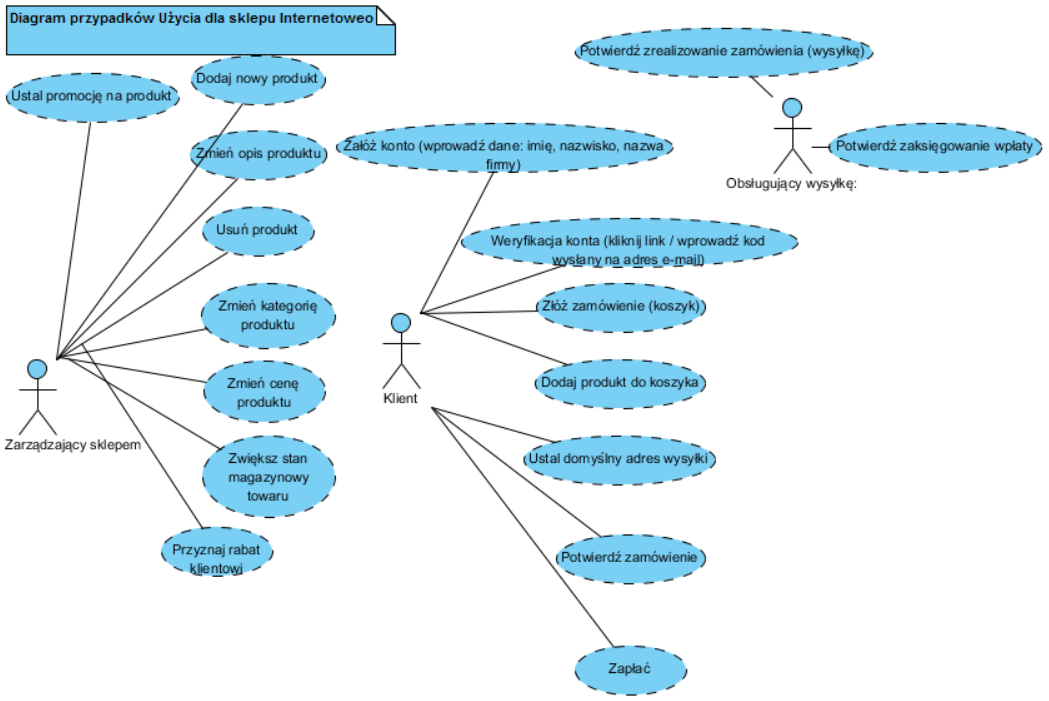
\includegraphics[width=15 cm] {fig/use_case_diagram}
	\caption{Diagram przypadków uycia}
	\label{fig:use_case_diagram}
\end{figure}
\subsection{Diagram klas}
\begin{figure}[H]
	\centering
	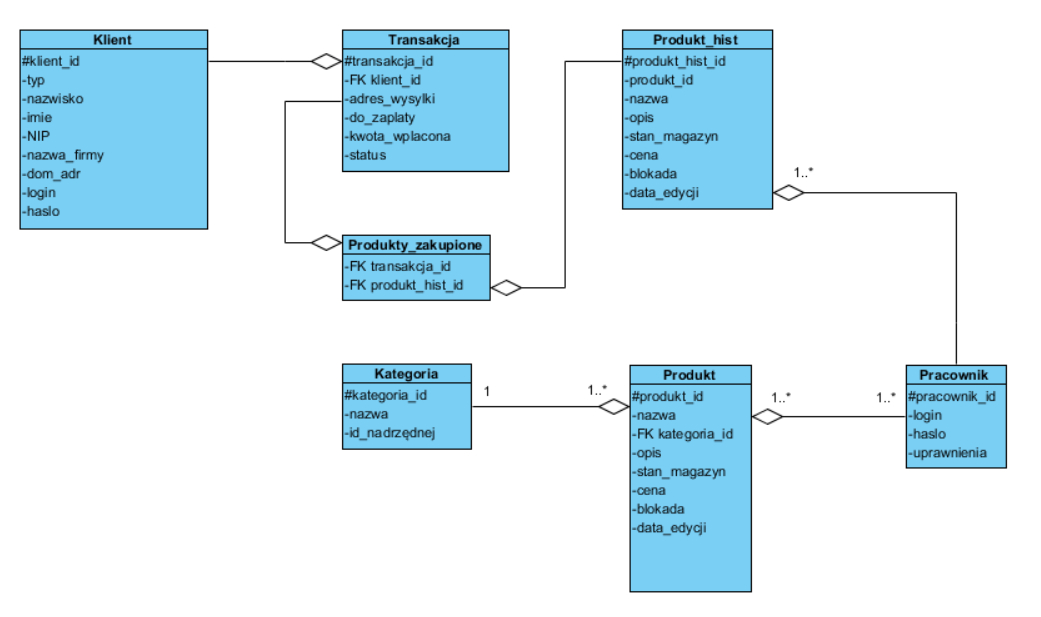
\includegraphics[width=15 cm] {fig/klasy}
	\caption{Diagram klas}
	\label{fig:diagram klas}
\end{figure}
\subsection{Wyjściowa funkcjonalność}

Sklep/seris internetowy z możliwością założenia konta użytkownika.
	
Rodzaje kont w serwisie:
	
Co najmniej jedno konto z uprawnieniami administratora z zastrzeżeniem że nie może usunąć własnego konta (zabezpieczenia aby w serwisie istniało konto administatora)

Konta pracowników którym można nadać odpowiednie uprawnienia dodawanie/usuwanie kategorii/produktów generowanie raportów sprzedaży. Konto pracownika może posiadać wszystkie uprawnienia lub tylko wybrane. Konto pracownika może być utworzone/skasowane tylko przez innego pracownika z uprawnieniami do zarządzania kontami pracowników.

Konta użytkowników. Standardowe konta użytkowników. Użytkownik ma prawo edytowania/zmiany swoich danych osobowych. Do rozróżniania użytowników wykorzystywane są ich unikalne loginy podawane przy rejestracji w serwisie.
Zasady tworzenia loginów:
\begin{enumerate}
\item Login musi być unikalny w bazie
\item Nie jest rozróżniana wielkość znaków w loginie np. ADMIN, admin, AdMin - traktowany jest jak jeden login
\end{enumerate}
Loginy są zapisywane w bazie, raz wykorzystany login nie może być użyty ponownie.

Użytkownik ma możliwość usunięcia konta z serwisu. w takim przypadku muszą zostać usunięte wszystkie jego dane osobowe. Zachowane zostają dane o przeprowadzonych z tym klientem transakcjach bez możliwości jego identyfikacji.



	
\section{Definiowanie tabel, wiezów integralnosci, perspektyw}

\subsection{Procedury}
\begin{enumerate}
\item \textbf{kategoria\_lista\_podrzednych}
\begin{verbatim}
BEGIN
DECLARE n INT;
SET n=1;
CREATE TEMPORARY TABLE podrzedne (`kategoria\_id` int(10) unsigned NOT NULL,`nazwa` varchar(30) COLLATE utf8\_polish\_ci NOT NULL,
`id\_nadrzednej` int(10) unsigned, `przetworzona` tinyint(1) DEFAULT 0);
CREATE TEMPORARY TABLE podrzedne2 (`kategoria\_id` int(10) unsigned NOT NULL,`nazwa` varchar(30) COLLATE utf8\_polish\_ci NOT NULL,
`id\_nadrzednej` int(10) unsigned, `przetworzona` tinyint(1) DEFAULT 0);

INSERT INTO podrzedne SELECT kategoria\_id, nazwa, id\_nadrzednej, 0 FROM kategoria WHERE kategoria\_id=id\_kat;

WHILE n>0 DO
INSERT INTO podrzedne2 SELECT kategoria\_id, nazwa, id\_nadrzednej, 0 FROM kategoria WHERE id\_nadrzednej IN (SELECT kategoria\_id FROM podrzedne WHERE przetworzona=0);
UPDATE podrzedne SET przetworzona=1;
INSERT INTO podrzedne SELECT * FROM podrzedne2;
TRUNCATE TABLE podrzedne2;
SELECT COUNT(*) FROM podrzedne WHERE przetworzona=0 INTO n;
END WHILE;

SELECT * FROM podrzedne;

DROP TEMPORARY TABLE podrzedne;
DROP TEMPORARY TABLE podrzedne2;
END
\end{verbatim}
\item menu\_drzewo\_kat
\begin{verbatim}
BEGIN
DECLARE kat\_id INT;
IF pkat\_id IS NOT NULL THEN
SET kat\_id = pkat\_id;
WHILE kat\_id IS NOT NULL DO
SELECT * FROM kategoria WHERE id\_nadrzednej=kat\_id;
SELECT id\_nadrzednej FROM kategoria WHERE kategoria\_id=kat\_id INTO kat\_id;
END WHILE;
END IF;
SELECT * FROM kategoria WHERE id\_nadrzednej IS NULL;
END
\end{verbatim}
\item produkt\_by\_kategoria
\begin{verbatim}
BEGIN
DECLARE n INT;
SET n=1;
CREATE TEMPORARY TABLE podrzedne (`kategoria\_id` int(10) unsigned NOT NULL, `przetworzona` tinyint(1) DEFAULT 0);
CREATE TEMPORARY TABLE podrzedne2 (`kategoria\_id` int(10) unsigned NOT NULL, `przetworzona` tinyint(1) DEFAULT 0);

INSERT INTO podrzedne VALUES(id\_kat,0);

WHILE n>0 DO
INSERT INTO podrzedne2 SELECT kategoria\_id, 0 FROM kategoria WHERE id\_nadrzednej IN (SELECT kategoria\_id FROM podrzedne WHERE przetworzona=0);
UPDATE podrzedne SET przetworzona=1;
INSERT INTO podrzedne SELECT * FROM podrzedne2;
TRUNCATE TABLE podrzedne2;
SELECT COUNT(*) FROM podrzedne WHERE przetworzona=0 INTO n;
END WHILE;

SELECT p.produkt\_id, p.nazwa, p.kategoria\_id, k.nazwa AS nazwa\_kat  FROM produkt p JOIN kategoria k USING(kategoria\_id) WHERE p.blokada=0 AND k.kategoria\_id IN (SELECT kategoria\_id FROM podrzedne);

DROP TEMPORARY TABLE podrzedne;
DROP TEMPORARY TABLE podrzedne2;
END
\end{verbatim}
\item produkt\_hist
\begin{verbatim}
BEGIN
DECLARE vprodukt\_id INT;
DECLARE poprz\_nazwa VARCHAR(50);
DECLARE poprz\_cena DECIMAL(10,2);
DECLARE poprz\_opis TEXT;
DECLARE poprz\_blokada TINYINT(1);
SELECT produkt\_id INTO vprodukt\_id FROM produkt\_edycja WHERE produkt\_edycja\_id=pprodukt\_edycja\_id;
SELECT poprz\_wartosc INTO poprz\_nazwa FROM produkt\_edycja WHERE produkt\_edycja\_id>pprodukt\_edycja\_id AND produkt\_id=vprodukt\_id AND kolumna='nazwa' ORDER BY produkt\_edycja\_id ASC LIMIT 1;
SELECT poprz\_wartosc INTO poprz\_cena FROM produkt\_edycja WHERE produkt\_edycja\_id>pprodukt\_edycja\_id AND produkt\_id=vprodukt\_id AND kolumna='cena' ORDER BY produkt\_edycja\_id ASC LIMIT 1;
SELECT poprz\_wartosc INTO poprz\_opis FROM produkt\_edycja WHERE produkt\_edycja\_id>pprodukt\_edycja\_id AND produkt\_id=vprodukt\_id AND kolumna='opis' ORDER BY produkt\_edycja\_id ASC LIMIT 1;
SELECT poprz\_wartosc INTO poprz\_blokada FROM produkt\_edycja WHERE produkt\_edycja\_id>pprodukt\_edycja\_id AND produkt\_id=vprodukt\_id AND kolumna='blokada' ORDER BY produkt\_edycja\_id ASC LIMIT 1;

SELECT COALESCE(poprz\_nazwa,nazwa) AS nazwa, COALESCE(poprz\_cena,cena) AS cena, COALESCE(poprz\_opis,opis) AS opis, COALESCE(poprz\_blokada,blokada) AS blokada FROM produkt WHERE produkt\_id=vprodukt\_id; 
END
\end{verbatim}
\end{enumerate}
\subsection{Funkcje}
Funkcje wykorzystane w projektowanej bazie danych

\begin{enumerate}
	\item ostatnia\_produkt\_edycja\_id
	\begin{verbatim}
	RETURN (SELECT MAX(`produkt\_edycja\_id`) FROM `produkt\_edycja` WHERE `produkt\_id`=produktid)
	\end{verbatim}
\end{enumerate}
\chapter{Interfejs - strona internetowa}

%Usuwa numeracje z naglowka. Zapewnia  dodanie do spisu tresci
\setcounter{secnumdepth}{-1}


%Gdy mamy dużą bibliografię to możemy wybierać pozycje,
%które cytujemy
%\nocite{ad-tg-80}

%Dodaje wszystkie pozycje z bibliografii
%\nocite{*}

%Po kazdym dodaniu nowej pozycji bibliograficznej
%z katalogu glownego uruchom: bibtex pracadyp
%\bibliographystyle{pdplain}
%\bibliography{tex/pracadyp}

\begin {thebibliography}{}
\bibitem{Balcerzak2005} Balcerzak J., Pansiuk J.: \emph{Wprowadzenie do kartografii matematycznej}, Warszawa, OWPW~2005.
\end {thebibliography}


\listoffigures

%\listoftables
\end{document}